\xhdr{Principals and agents.} There are two principals and $T$ agents. We denote them, resp., principal $i\in \{1,2\}$ and agent $t\in [T]$,
where $[T] := \{1,2\LDOTS T\}$.
%The game proceeds in $T$ rounds.

In each round $t\in [T]$, the following  interaction takes place. Agent $t$ arrives and chooses a principal $i_t\in \{1,2\}$. The principal chooses action $a_t\in A$, where $A$ is a fixed set of actions.%
\footnote{We use `action' and `arm' interchangeably, as common in the literature on multi-armed bandits.}
The agent experiences this action and receives an associated reward $r_t\in \{ 0,1\}$, which is then observed by the principal. We posit \emph{stochastic rewards}: whenever a given action $a\in A$ is chosen, the reward is an independent draw from Bernoulli distribution with mean $\mu_a$. In particular, the mean rewards $\mu_a$, as well as the action set $A$, are the same for both principals and all rounds. The mean rewards are initially not known to anybody. The principals are completely unaware of the rounds when the opponent is chosen.



% (which is the same for both principals and all rounds)

Thus, each principal follows the protocol of \emph{multi-armed bandits} (henceforth, \emph{MAB}). In each round when it is chosen, it chooses an arm from $A$ and observes a reward for this action. It does not observe anything else, particularly rewards for other actions.

Each principal $i$ commits to an MAB algorithm \alg[i] before round $1$, and uses this algorithm throughout the game. The algorithm proceeds in time-steps:
%\footnote{These time-steps will sometimes be referred to as \emph{local steps/rounds}, so as to distinguish them from ``global rounds" defined before. We will omit the global vs. local distinction when clear from the context.}
each time it is called, it outputs an arm from $A$, and inputs a reward for this action. The algorithm is called only in game rounds when principal $i$ is chosen.
When the distinction between algorithm's time-steps and game rounds is unclear from the context, we will refer to them as, resp., \emph{local steps/rounds} and \emph{global rounds}.

\newcommand{\est}{\mathtt{EST}}

%\gaedit{\footnote{While our model assumes that agents have correct beliefs about the performance of the algorithms, only the beliefs themselves matter and so our results hold as long as all agents have the same initial beliefs, even if they are not aligned with the true prior.}}

\xhdr{Agent response.} Each agent $t$ forms a reward estimate $\est_i(t)\in [0,1]$ for each principal $i$. (What these estimates are, and how much the agents know in order to form them, depends on the Bayesian vs. frequentist model variant.)
The reward estimates determine the choice of the principal. Specifically, agent $t$ chooses principal $1$ with probability
\begin{align}\label{eq:model-f}
p_t = \respF\rbr{ \est_1(t) - \est_2(t) },
\end{align}
where $\respF:[-1,1]\to [0,1]$ is the \emph{response function}, same for all agents. We assume that $\respF$ is monotonically non-decreasing, is larger than $\nicefrac12$ on the interval $(0,1]$, and smaller than $\nicefrac12$ on the interval $[-1,0)$. We consider three variants for $\respF$, depicted in  \reffig{fig:response-functions}:

\begin{figure}[t]
\begin{center}
  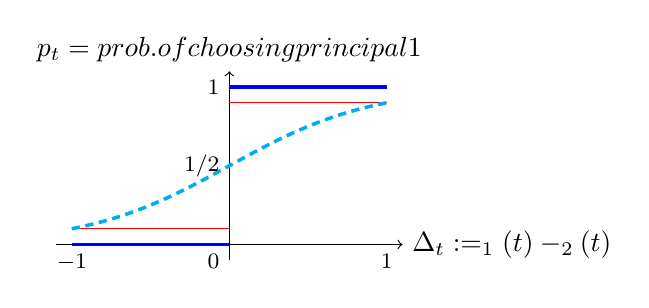
\begin{tikzpicture}[scale=2.0]
    \draw[->] (-1.1,0) -- (1.1,0) node[right]
    {$\Delta_t := \est_1(t) - \est_2(t)$};
    \draw[->] (0,-0.1) -- (0,1.1) node[above]
        {$p_t = \text{prob. of choosing principal 1}$};
    \draw[scale=1.0,domain=-1:0,smooth,variable=\q,blue, line width=0.50mm] plot ({\q},{0});
    \draw[scale=1.0,domain=0:1,smooth,variable=\q,blue,line width=0.50mm] plot ({\q},{1});
    \draw[scale=1.0,domain=-1:0,smooth,variable=\y,red]  plot ({\y},{0.1});
    \draw[scale=1.0,domain=0:1,smooth,variable=\y,red]  plot ({\y},{0.9});
    \draw[scale=1.0,domain=-1:1,smooth,variable=\y,cyan, line width=0.45mm, dash pattern=on 3pt off 2pt]  plot ({\y},{1/(1 + 1/(9^\y))});
    % \node[above, blue] at (0.5, 0.5) {\footnotesize $2 q (1 - q)$};
     \node[left] at (0, 0.5) {\footnotesize $1/2$};
     \node[left] at (0, 1) {\footnotesize $1$};
     \node[below left] at (0, 0) {\footnotesize $0$};
     \node[below ] at (1, 0) {\footnotesize $1$};
     \node[below ] at (-1, 0) {\footnotesize $-1$};
  \end{tikzpicture}
\end{center}
\caption{The models for $\respF$: \HardMax is thick blue, \HardMaxRandom is red, and \SoftMaxRandom is dashed.}
\label{fig:response-functions}
\end{figure}

\begin{OneLiners}
\item \HardMax: $\respF$ equals $0$ on the interval $[-1,0)$ and $1$
  on the interval $(0,1]$. In words, a \HardMax agent
  deterministically chooses a principal with a higher reward estimate.

\item \HardMaxRandom:
    % $\respF$ equals $\eps$ on the interval $[-1,0)$ and $1-\eps'$ on the interval $(0,1]$, where $\eps,\eps'\in (0,\tfrac12)$ are some positive constants. In words, each agent is a \HardMax agent with probability $1-\eps-\eps'$, and with the remaining probability she makes a random choice.
    $\respF$ equals $\eps_0$ on the interval $[-1,0)$ and $1-\eps_0$ on the interval $(0,1]$, for some constant $\eps_0\in (0,\tfrac12)$. In words, each agent is a \HardMax agent with probability $1-2\eps_0$, and makes a random choice otherwise.

\item \SoftMaxRandom: $\respF$  lies in $[\eps_0,1-\eps_0]$, breaks ties fairly, and has a bounded derivative around $0$ (see Definition~\ref{def:SoftMax} for a formal definition). Intuitively, $\respF$ is a smoothed version of \HardMaxRandom, without a sharp threshold therein.
\end{OneLiners}

\HardMaxRandom and \SoftMaxRandom agents can be interpreted in several ways. First, they make mistakes, due to lack of awareness or interest. Second, they give some chance to the non-preferred principal, due to curiosity or a behavioral effect like probability matching.
%\gaedit{make mistakes due to being oblivious to the principals' reputation, due to lack of awareness or interest. \HardMaxRandom models users as either being aware of the reputation or not, whereas \SoftMaxRandom models user mistakes as following a smooth density.}
Third, they can be realized as a distribution over more ``basic" agent types. Indeed, the \HardMaxRandom distribution is a mixture of \HardMax and ``random agents" (which choose a principal uniformly at random). The latter can be interpreted as consumers that are completely oblivious to principals' reputation.
%, due to the lack of awareness or interest.}
One can obtain a \SoftMaxRandom response function using agent types that choose a principal $i$ with a largest reward estimate $\est_i$, unless $|\est_1-\est_2|$ is upper-bounded by some parameter $\theta$, in which case they choose uniformly. Then, we obtain \SoftMaxRandom as a mixture of random agents and these ``$\theta$-\HardMax'' agents, for a suitable distribution over $\theta$.


% \asedit{(We assume $\respF(-1)+\respF(1)=1$ in \HardMaxRandom and \SoftMaxRandom only to simplify notation.)}

%We say that $\respF$ is \emph{symmetric} if $\respF(-x)+\respF(x)=1$ for any $x\in [0,1]$. This implies \emph{fair tie-breaking}: $\respF(0)=\tfrac12$.

\xhdr{Bayesian vs. frequentist.}
We consider two model variants, Bayesian and frequentist (which we use, resp., for theoretical results and numerical simulations). The main difference between the two concerns the agents' reward estimates $\est_i(t)$.

\begin{OneLiners}
\item In the \emph{\TheoryModel}, the mean reward vector $\mu = (\mu_a:\; a\in A)$ is drawn from a common Bayesian prior $\priorMu$. Each agent knows its global round $t$, but not the performance signals such as the current market shares. Her reward estimates are defined as posterior mean rewards:
        $\est_i(t) = \PMR_i(t) := \E\sbr{ r_t\mid i_t = i}$
    for each principal $i$, where the agent knows $t$, the principals' algorithms, $\priorMu$, and $\respF$.
%\footnote{Agents do the Bayesian update knowing $t$, the principals' algorithms, the prior $\priorMu$, and $\respF$.}

%Agents know the principals' algorithms.\gaedit{\footnote{While our model assumes that agents have correct beliefs about the performance of the algorithms, only the beliefs themselves matter and so our results hold as long as all agents have the same initial beliefs, even if they are not aligned with the true prior.}}

\item In the \emph{\ExptsModel}, agents' reward estimate for a given principal is the average reward of the last $M$ agents that chose this principal. We call it \emph{reputation score}, and interpret it as the current reputation. To make it meaningful initially, each principal enjoys a ``warm start": additional $T_0$ agents arrive before the game starts, and interact with the principal as described above.

\end{OneLiners}

\xhdr{Competition game.}
Some of our results explicitly study the game between the two principals, termed the \emph{competition game}. We model it as a simultaneous-move game: before the first agent arrives, each principal commits to an MAB algorithm. (Since MAB algorithms can be randomized, we make no distinction between pure and mixed strategies.) Principals are risk-neutral; their utility is defined as their market share, \ie the number of agents they attract. Thus, they aim to select the algorithm that maximizes their expected market share.

%Principal's utility is defined as the market share, \ie the number of agents that chose this principal. Principals are risk-neutral and aim to maximize their expected utility.


\xhdr{Extensions.} The \TheoryModel admits several extensions, detailed in Section~\ref{sec:theory-extensions}. First, all/most results extend to arbitrary reward distributions, allow reward-dependent utility, and carry over to a more general version of multi-armed bandits. Second, agents could have beliefs on $(\alg[1],\alg[2],\priorMu,\respF)$ that need not be correct; then, all results carry over with respect to these beliefs.
%Third, all results carry over \asmargincomment{check}  if each agent $t$ has a prior on her arrival time $t$, rather than know it exactly.
Third, we can handle a limited amount of non-stationarity in $\respF$ for the \HardMaxRandom and \SoftMaxRandom decision rules. Finally, the main result on \HardMax extends to time-discounted utilities.


\subsection{Discussion}
\label{sec:discussion}

Now that we laid out our model, let us discuss several aspects thereof that are unclear from the bare definitions. In particular, we flesh out several points made in the Introduction.

Reflecting reality, we posit that the exploration strategies available to the principals are ``non-strategic" in nature. Even though the principals play a multi-step game, they do not react to each other's moves or to the agents' strategic choices. This is how industry approaches exploration algorithms, and for several good reasons. "Non-strategic" exploration is well-studied in machine learning, and yet it remains a very complex and actively studied subject in research. Even the seemingly simple algorithms are not straightforward to deploy in practice, and require a substantial investment in infrastructure \cite[\eg see the discussions in][]{DS-arxiv}. Responding to the competition represents another layer of complexity which has not been previously studied in this context, to the best of our knowledge, let alone made even remotely practical. Besides, the competitor's exploration strategy is typically not public, and understanding its exploration behavior via observations appears challenging even as a  research problem.%
\footnote{Principals could potentially react to the market share or (the difference in) reputation scores. However, baking these signals into one's exploration strategy runs the risk of over-interpreting our competition model, as they may change for exogenous reasons. Alternatively, one could use such signals, as well as the intuitions coming from this paper, to guide the platform's decisions regarding exploration.}


%\gaedit{Finally, the assumption that firms commit to the algorithms at the start of the game deserves further justification. We impose this commitment assumption since it is more realistic than considering dynamic strategies and algorithms are, by definition, a commitment to a set of rules. In many contexts where such exploration algorithms are typically deployed, consumers arrive at such a rapid volume that it it is infeasible to consider a firm dynamically adapting its algorithm to each consumer that arrives. Indeed, \cite{DS-arxiv} points out how difficult it is to deploy standard exploration algorithms in practice and such dynamic strategies are substantially more difficult to deploy in practice. While it is possible to consider share-adaptive algorithms that would still keep the commitment assumption but allow for indirect dynamic responses to market conditions, such algorithms do not exist currently in the literature but are a good avenue for future work.}



Our models are stylized in several important  respects. Firms compete only on the quality of service, rather than, say, pricing or the range of products. Agents are myopic: they do not worry about how their actions impact their future utility.\footnote{So, agents do not attempt to learn over time, game future agents, or manipulate the principals' learning algorithms. This is arguably typical in practice, in part because one agent's influence tends to be small.}  Various performance signals available to the users, from personal experience to word-of-mouth to consumer reports, are abstracted as persistent ``reputation scores" reflecting the current reputation, and further simplified to average performance over a sliding time window.

We consider two extremes: a simple Bayesian model with full Bayesian rationality and no performance signals, and a simple frequentist model with reputation scores and no prior knowledge or beliefs. For the theoretical results, the ``no-performance-signals" assumption makes agents' behavior independent of a particular realization of the prior. Therefore, we summarize each learning algorithm via its Bayesian-expected rewards, not worrying about its detailed performance on particular realizations of the prior.  Such summarization is essential for formulating lucid and general analytic results, let alone proving them. It is unclear how to incorporate performance signals in a theoretically tractable model. For the numerical results, the \ExptsModel accounts for competition in a more direct way,
% \gaedit{by positing a more realistic model of consumer behavior that does not
not requiring users to have direct information on the algorithms deployed or the bandit problem faced by the firms. It further allows us to separate reputation vs. data advantage and makes our model amenable to numerical simulations.
%(Whereas simulating the intricate interplay of learning dynamics and Bayesian priors appears computationally intractable, see Footnote~\ref{fn:Tsquared}.)


On the machine learning side, our model captures big, qualitative differences between bandit algorithms, building on the well-established intuition in the literature. Comparisons between bandit algorithms are generally somewhat subtle, as some algorithms may be better for some problem instances and/or time intervals, and worse for some others. In particular, ``better" algorithms are better in the long run, but could be worse initially. We focus on a standard model of stochastic bandits. In Appendix~\ref{app:bg}, we present sufficient background on this model, accessible to non-specialists. However, we are less interested in state-of-art algorithms for realistic applications.

Bandit rewards are not discounted with time, reflecting the fact that non-discounted, regret-minimizing formulations has been prevalent in the bandits literature over the past two decades \citep{slivkins-MABbook,LS19bandit-book}, and better correspond to practical deployments \citep[\eg][]{DS-arxiv}. Also, the distinctions between better and worse bandit algorithms are not as well-understood under time-discounting.

